\section{Results}

\subsection{Evaluate trait reconstruction and optimum research}

To test the capacity of Foucart Correspondence Analysis to reconstruct the latent traits, we measure the average correlation of the first axis with the first trait and of the second axis with the second trait.

\subsubsection{Effect of the number of interactions ($n_{inter\_tot}$)}

\begin{figure}[H]
    \centering
    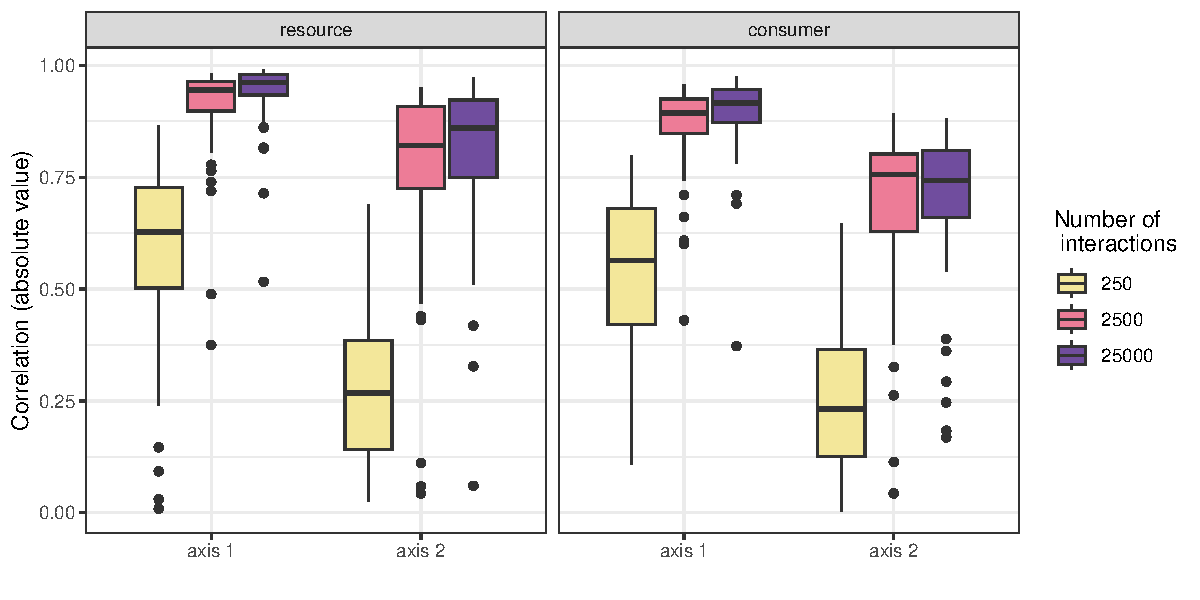
\includegraphics[width=1\linewidth, , trim=0cm 3cm 0cm 2cm, clip]{FIGURES/ninter.pdf}
    \caption{Evaluation of the reconstruction of the trait depending on the total number of interactions observed (50 consumer species, 50 resource species, $n_{frame} = 5$, $\delta =  0.2$, $trait\_ratio = 0.7$, $\mu_{tol\_env} = 0.5$ and $\mu_{tol\_trait} = 0.1$)}
    \label{fig:ninter}
\end{figure}

As expected, the recovery of the traits increases with the number of interactions sampled across all the networks. Specifically, trait recovery is significantly higher when there is an equivalent of one observation per potential interaction. With ten times more observation, the improvement is marginal. This can be explained by the diminution of the stochasticity due to the sampling effect.


\subsubsection{Joint influence of the number of sampled locations and the environmental tolerance ($n_{frame} \times \mu_{tol\_env}$)}

\begin{figure}[H]
    \centering
    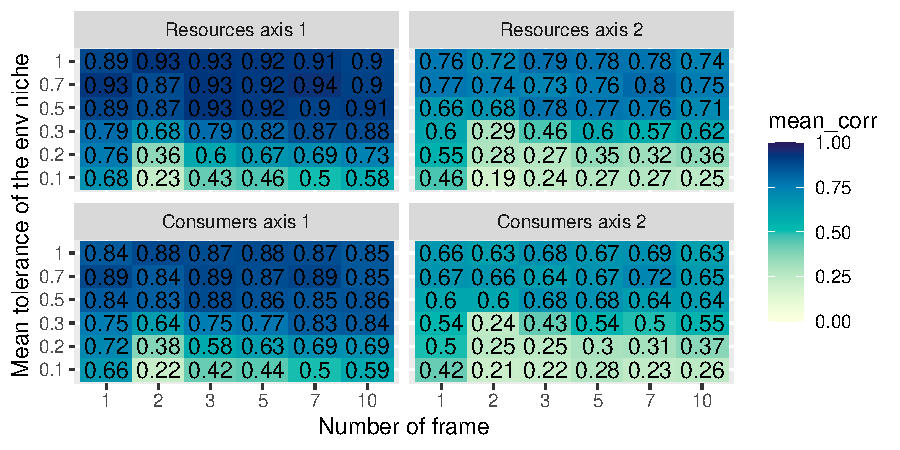
\includegraphics[width=0.75\linewidth]{FIGURES/frame_env.pdf}
    \caption{Evaluation of the reconstruction of the trait depending on the crossed effect of the number of sites and the environmental tolerance (50 consumer species, 50 resource species, $n_{inter\_tot} = 2500$, $\delta =  0.2$, $trait\_ratio = 0.7$ and $\mu_{tol\_trait} = 0.1$)}
    \label{fig:frame_env}
\end{figure}

Examining the joint influence of the number of frames and the environmental tolerance depicted in Figure \ref{fig:frame_env}, we observe that reconstruction is better for low environmental tolerance values when there is only one sampling location. This is because a single sampled location is placed in the middle of the environmental gradient. With two locations, they are positioned at the two extremities of the gradient. When more locations are included, they are evenly spaced with the first one at the beginning and the last one at the end of the gradient. 
Since all optima are included in the range of the environmental gradient ($0 < \mu_{tol\_env} < 1$), placing the sampled location in the middle of the gradient results in most species being represented. However, with two locations, some species tend to be missed in each network, leading to nearly disjoint sets of species in the networks. This disjointedness is reinforced by the sampling effect getting stronger (as the total number of observations is fixed), making it challenging for the Foucart CA to find common axes for both networks and explaining the drop in trait recovery.

Increasing the number of frames leads to intermediate networks and a finer description of all the species across the environmental gradient, which explains the better performance of trait recovery. Similarly, a higher mean environmental tolerance, results in a more uniform species abundances across the different sampling locations, thus enhancing the trait recovery.


\subsubsection{Effect of the weight given to trait matching ($\delta$)}

\begin{figure}[H]
    \centering
    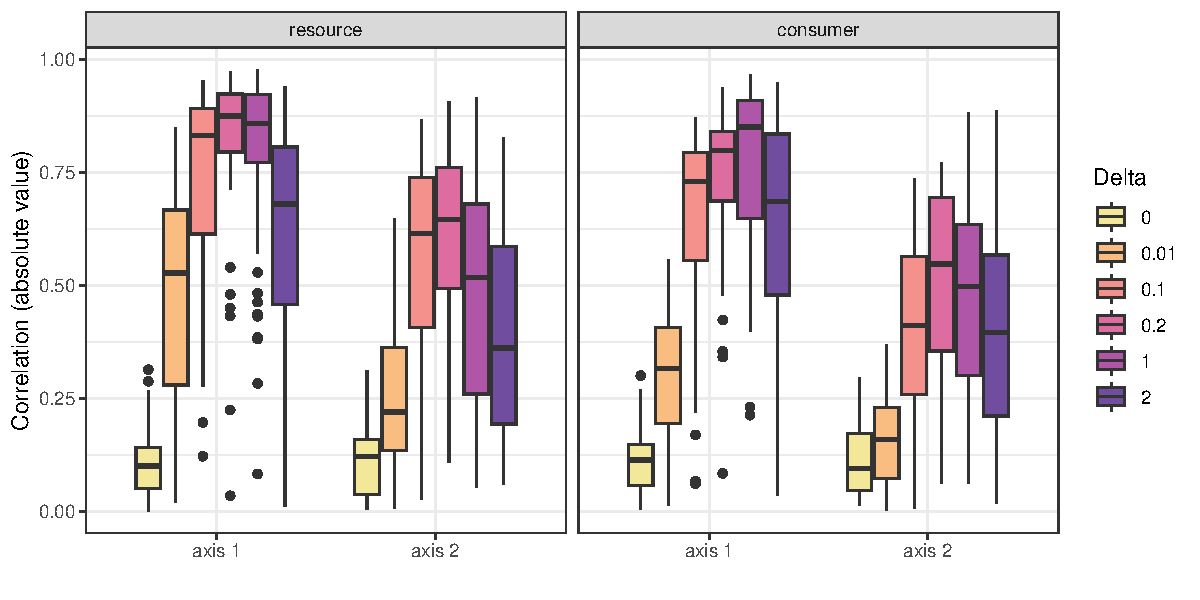
\includegraphics[width=1\linewidth, trim=0cm 3cm 0cm 2cm, clip]{FIGURES/delta.pdf}
    \caption{Evaluation of the reconstruction of the trait depending on the weight given to trait matching (delta) (50 consumer species, 50 resource species, $n_{inter\_tot} = 2500$, $n_{frame} = 5$,$trait\_ratio = 0.7$, $\mu_{tol\_env} = 0.5$ and $\mu_{tol\_trait} = 0.1$)}
    \label{fig:delta}
\end{figure}

Trait recovery increases with the weight given to trait matching ($\delta$) up to $\delta = 0.2$ after which it decreases when the trait matching is too important ($\delta = 2)$. Increasing the weight given to trait matching initially reduces the stochasticity caused by the mean-field effect of the abundances. However, the trait recovery decreases beyond a certain point. This decline might be due to a decreasing diversity of the species in the interaction profile, i.e., only the species present and with the best trait matching will be observed. Thus it will be hard to find common axes.



\subsubsection{Effect of the relative weight given to the traits ($trait\_ratio$)}

\begin{figure}[H]
    \centering
    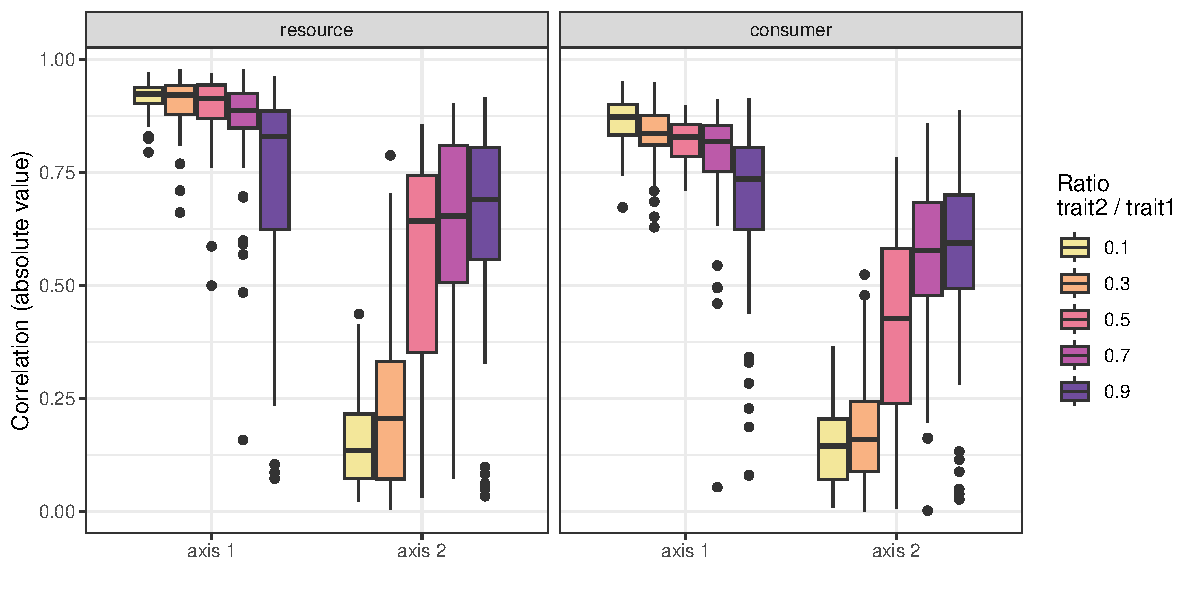
\includegraphics[width=1\linewidth, trim=0cm 3cm 0cm 2cm, clip]{FIGURES/ratio.pdf}  % d b g h
    \caption{Evaluation of the reconstruction of the trait depending on the ratio between the first and the second trait (50 consumer species, 50 resource species, $n_{inter\_tot} = 2500$, $n_{frame} = 5$, $\delta =  0.2$, $\mu_{tol\_env} = 0.5$ and $\mu_{tol\_trait} = 0.1$)}
    \label{fig:trait_ratio}
\end{figure}

When most of the weight is given to the first trait, the correlation between the first axis and the first trait is the highest, while the correlation between the second axis and the second trait is the lowest. As the weight given to the second trait increases, the correlation between the first axis and the first trait decreases, and the correlation between the second trait and the second axis increases, although the recovery for trait 2 does not reach the same level as trait 1. This discrepancy arises because axis 1 is a composite that holds information about both traits. The overall recovery of the trait information remains constant. However, as we increase the weight given to the second trait, axis 1 increasingly reflects information about the second trait while the second axis becomes more representative of the first trait.


\subsubsection{Effect of the trait tolerance ($\mu_{tol\_trait}$)}

\begin{figure}[H]
    \centering
    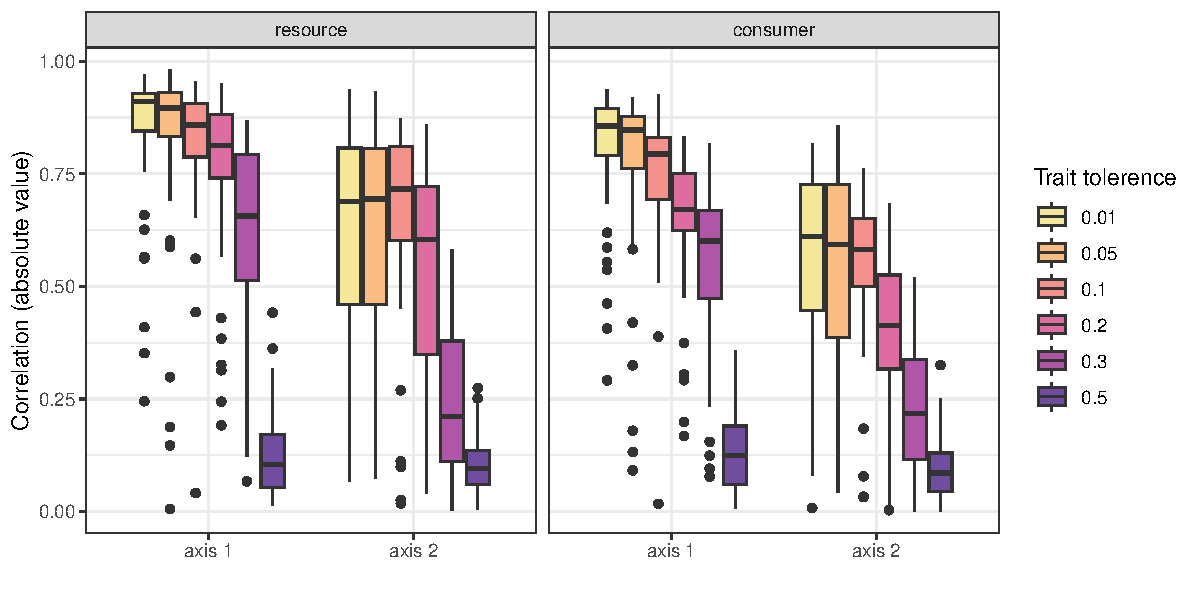
\includegraphics[width=1\linewidth, trim=0cm 3cm 0cm 2cm, clip]{FIGURES/trait.pdf}
    \caption{Evaluation of the reconstruction of the trait depending on trait tolerance (50 consumer species, 50 resource species, $n_{inter\_tot} = 2500$, $n_{frame} = 5$, $\delta =  0.2$, $trait\_ratio = 0.7$ and $\mu_{tol\_env} = 0.5$)}
    \label{fig:tol_trait}
\end{figure}

The recovery of the traits decreases with increasing trait tolerance ($\mu_{tol\_trait}$). Notably, the trait recovery drastically decreases when $\mu_{tol\_trait}$ exceeds  $0.2$.This may be explained by the fact that the sharper peak of the optimum of the traits indicates more specialized species, making it easier to accurately locate the trait optimum. However, with higher trait tolerance, the probability of slightly mispositioning the trait optimum increases. Such mispositioning can make minor switches in the trait order and thus significantly reduce the correlation.



\subsection{Rewiring estimation: correlation of the $\beta$ diversity contribution ($\Delta_{OS}$) and the position's variance in the Foucart Correspondence Analysis}

Now that Foucart CA is known to be able to reconstruct the traits (which is analogous to the interaction profile), we will study the correlation between the and the individual contribution to the $\beta$ diversity of link turnover of \citet{toju_interaction_2024} (which is currently the only way to compute the species contribution to rewiring) and the position's variance in Foucart CA. 
We will also assess the impact of environmental and trait tolerance on the position's variance in Foucart CA.

\begin{figure}[H]
    \centering
    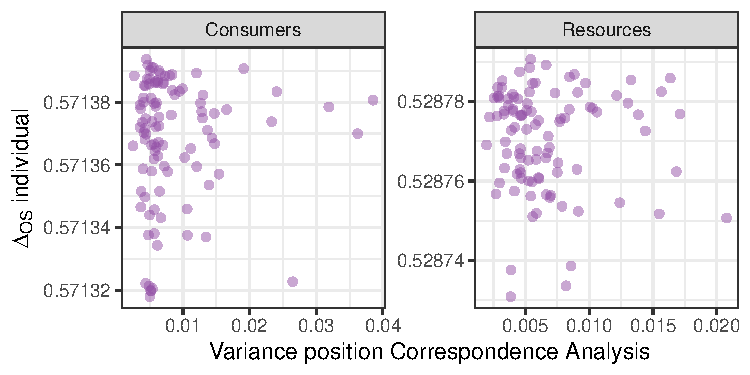
\includegraphics[width=0.75\linewidth]{FIGURES/rewiring.pdf}
    \caption{Comparison of rewiring estimation with the correspondence analysis and with the $\beta$ diversity rewiring contribution (100 consumer species, 100 resource species, $n_{inter\_tot} = 10000$, $n_{frame} = 5$, $\delta =  0.2$, $trait\_ratio = 0.7$, $\mu_{tol\_env} = 0.5$and $\mu_{tol\_trait} = 0.1$)}
    \label{fig:toju}
\end{figure}

There appears to be no correlation between the variance of position in the Correspondence Analysis and the individual contribution to the $\beta$ diversity of link turnover the way it is computed in the article of \citet{toju_interaction_2024}. This lack of correlation is observed for both consumers and resources. The range of the $\Delta_{OS}$ is approximately of order $10^{-5}$ while the variance in position has a range of order $0.02$.



\subsection{Impact of the species characteristics on the position's variance in the Foucart Correspondence Analysis}

\subsubsection{Impact of the environmental tolerance}

\begin{figure}[H]
    \centering
    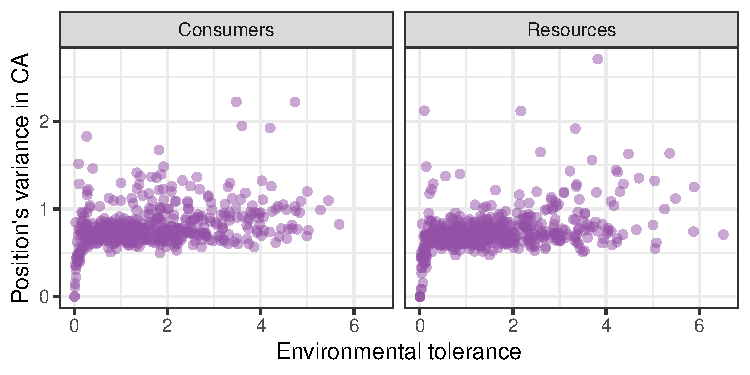
\includegraphics[width=0.75\linewidth]{FIGURES/impact_env.pdf}
    \caption{Effect of the environmental tolerance on the observed position's variance in the CA (500 consumer species, 500 resource species, $n_{inter\_tot} = 25000$, $n_{frame} = 10$, $\delta =  0.2$, $trait\_ratio = 0.7$, $\mu_{tol\_env} = 0.5$ and $\mu_{tol\_trait} = 0.1$)}
    \label{fig:effect_env}
\end{figure}

The position's variance increases with the environmental tolerance ($\mu_{tol\_env}$) when this one is low ($\mu_{tol\_env} < 0.5$). Beyond this threshold, the position's variance no longer increases with the environmental tolerance and stabilizes at $1$. 

\subsubsection{Impact on the trait tolerance}

\begin{figure}[H]
    \centering
    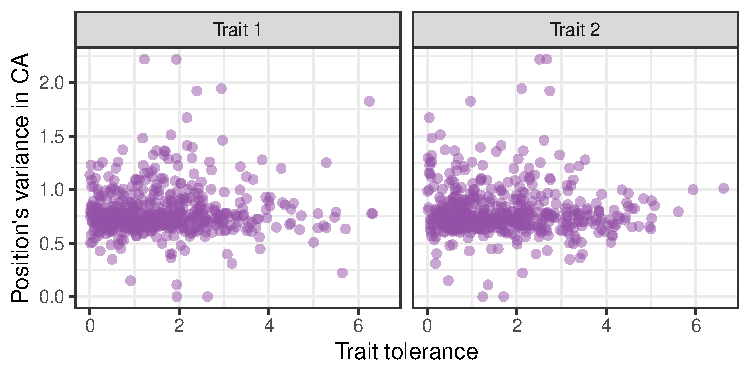
\includegraphics[width=0.75\linewidth]{FIGURES/impact_trait_tol.pdf}
    \caption{Effect of the trait tolerance on the observed position's variance in the CA (500 consumer species, 500 resource species, $n_{inter\_tot} = 25000$, $n_{frame} = 10$, $\delta =  0.2$, $trait\_ratio = 0.7$, $\mu_{tol\_env} = 0.5$ and $\mu_{tol\_trait} = 0.1$)}
    \label{fig:effect_trait}
\end{figure}

There appears to be no significant relationship between trait tolerance ($\mu_{tol\_trait}$) and the variance in the correspondence analysis. The position's variance remains stable at around $0.9$.